\label{chap:arch}
\subsection{Hardware}

The processing power and wireless capability of the wireless sensor nodes are provided by an Atmel
ZigBit 900MHZ RF module. It contains an ATmega 1281V 8-bit microcontroller connected to an
AT86RF212 RF Transceiver via a SPI interface. The Atmega 1281V is an low power 8 bit microcontroller
that is connected to the onboard sensors of the node. In order to be able to transmit or secure the
data, the microcontroller will communicate with the RF Transceiver. The Transceiver controller is a very low power chip,
capable of sending data up to 6 km. Also, the Transceiver contains a security module compatible
with AES-128. It supports hardware encryption and decryption for AES 128 ECB, but but for the AES
128 CBC it is available only the hardware encryption.


\begin{figure}[ht] \centering
  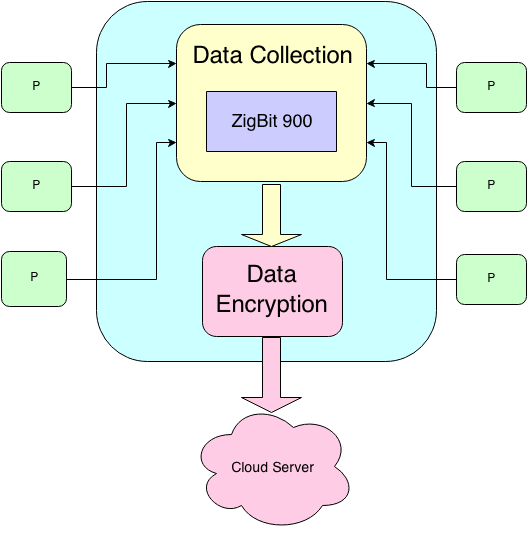
\includegraphics[width=0.5\textwidth]{img/wsn-soa-system-arch.png}
  \caption{System Architecture}
\end{figure}

\subsection{Software}

From the software perspective, the architecture is composed of three modules:
\begin{itemize}
\item data module, that
collects information from the sensors,
\item encryption module,
\item communication module.
\end{itemize}

Since the transceiver module is separated from the controller, from an efficiency perspective, it 
would be preferable to implement AES ECB and CBC algorithms as software services directly on the 
controller. Using this method, the transceiver shall be kept most of the time in an idle state, 
and the only component which will actively operate and drain the battery is the controller itself.
While the controller is one of the components which a high power consumption rate, the implementation 
will contain optimizations meant to keep the number of encryption operations performed to a minimum.
Moreover, it is important to filter data before packageing and sending it, in order to further 
reduce the number of encryption and decryption operations which the microcontroller of a node has 
to perform.

Overall, given the available hardware resources and architecture, the proposed implementation offers 
a software solution for ensuring data security and it also uses encryption methods which can easily 
be replaced with AES ones if ported on an hardware architecture in which the transceiver is 
incorporated in the microcontroller.
